\let\negmedspace\undefined
\let\negthickspace\undefined
\documentclass[journal]{IEEEtran}
\usepackage[a4paper, margin=10mm, onecolumn]{geometry}
%\usepackage{lmodern} % Ensure lmodern is loaded for pdflatex
\usepackage{tfrupee} % Include tfrupee package

\setlength{\headheight}{1cm} % Set the height of the header box
\setlength{\headsep}{0mm}  % Set the distance between the header box and the top of the text

\usepackage{gvv-book}
\usepackage{gvv}
\usepackage{cite}
\usepackage{amsmath,amssymb,amsfonts,amsthm}
\usepackage{algorithmic}
\usepackage{graphicx}
\usepackage{float}
\usepackage{textcomp}
\usepackage{xcolor}
\usepackage{txfonts}
\usepackage{listings}
\usepackage{enumitem}
\usepackage{mathtools}
\usepackage{gensymb}
\usepackage{comment}
\usepackage[breaklinks=true]{hyperref}
\usepackage{tkz-euclide} 
\usepackage{listings}
% \usepackage{gvv}                                        
\def\inputGnumericTable{}                                 
\usepackage[latin1]{inputenc}                                
\usepackage{color}                                            
\usepackage{array}                                            
\usepackage{longtable}                                       
\usepackage{calc}                                             
\usepackage{multirow}                                         
\usepackage{hhline}                                           
\usepackage{ifthen}                                           
\usepackage{lscape}
\usepackage{tikz}
\usetikzlibrary{patterns}

\begin{document}

\bibliographystyle{IEEEtran}
\vspace{3cm}

\title{9.2.31}
\author{ee25btech11063-vejith}

\maketitle
% \maketitle
% \newpage
% \bigskip
{\let\newpage\relax\maketitle}
\renewcommand{\thefigure}{\theenumi}
\renewcommand{\thetable}{\theenumi}
\setlength{\intextsep}{10pt} % Space between text and floats
\textbf{Question}\\
Find the area of the region bounded by the curve y$^2$=4x and x$^2$=4y\\
\textbf{Solution}:\\
\begin{table}[h!]    
  \centering
  \begin{tabular}{|c|c|}
\hline
\textbf{Name} & \textbf{Value} \\ \hline
$\vec{A}$ & $\myvec{2 & 1 \\0 & 3}$ \\ \hline
\end{tabular}

  \caption{Variables Used}
  \label{}
\end{table}\\
The equation of a parabola in Matrix form is
\begin{align}
\vec{x}^\top\vec{V}\vec{x} + 2\vec{u}^\top\vec{x} + f = 0
\end{align}
For y$^2$=4x
\begin{align}
    \vec{V_1}=\begin{pmatrix}
        0 & 0\\
        0 & 1
    \end{pmatrix}\\
    \vec{u_1}=-2\vec{e_1}=\myvec{-2\\0}\\
    f_1=0
\end{align}
For x$^2$=4y
\begin{align}
    \vec{V_2}=\begin{pmatrix}
        1 & 0\\
        0 & 0
    \end{pmatrix}\\
    \vec{u_2}=-2\vec{e_2}=\myvec{0\\-2}\\
    f_2=0
\end{align}
The intersection of two conics with parameters $\vec{v_i}$,$\vec{u_i}$,f$_i$ ,i=1,2 is defined as 
\begin{align}
\vec{X}^{T}\,(\vec{V}_{1} + \mu \vec{V}_{2})\vec{X} + 2(\vec{u_1} + \mu \vec{u_2})^{T}\vec{X} \;+\; (f_{1} + \mu f_{2}) \;=\; 0
\end{align}
\begin{align}
\implies \left|
\begin{array}{cc}
\mathbf{V}_1 + \mu \mathbf{V}_2 & \mathbf{u}_1 + \mu \mathbf{u}_2 \\[6pt]
(\mathbf{u}_1 + \mu \mathbf{u}_2)^{\mathrm{T}} & f_1 + \mu f_2
\end{array}
\right| = 0
\end{align}
\begin{align}
    \implies 
\left|
\begin{array}{ccc}
\mu & 0 & -2 \\[6pt]
0 & 1  & -2\mu \\[6pt]
-2 & -2\mu & 0
\end{array}
\right| = 0 \\
\implies \left|
\begin{array}{ccc}
\mu & 0 & -2 \\[6pt]
0 & 1  & -2\mu \\[6pt]
-2 & -2\mu & 0
\end{array}
\right| &\xleftrightarrow{R_3 \leftrightarrow R_3 + \frac{2}{\mu}\times R_1} \left|
\begin{array}{ccc}
\mu & 0 & -2 \\[6pt]
0 & 1  & -2\mu \\[6pt]
0 & -2\mu & -\frac{4}{\mu}
\end{array}
\right|\\
&\xleftrightarrow{R_3 \leftrightarrow R_3 + 2\mu \times R_2} \left|
\begin{array}{ccc}
\mu & 0 & -2 \\[6pt]
0 & 1  & -2\mu \\[6pt]
0 & 0 & -(\frac{4}{\mu} +4 \mu ^2)
\end{array}
\right| =0\\
\implies -(4 + +4 \mu ^3)=0\\
\implies \mu=-1
\end{align}
substituting the value of $\mu$=-1 in (8) we get points of intersection as 
\begin{align}
    \vec{x_1}=\myvec{0\\0} \\
    \vec{x_2}=\myvec{4\\4}
\end{align}
Area of the desired region is given by
\begin{align}
A &= \int_{0}^{4}2\sqrt{x}-\frac{x^2}{4}dx\\
A &= \frac{32}{3}-\frac{16}{3}\\
A &= \frac{16}{3}
\end{align}
\begin{figure}[h!]
    \centering
    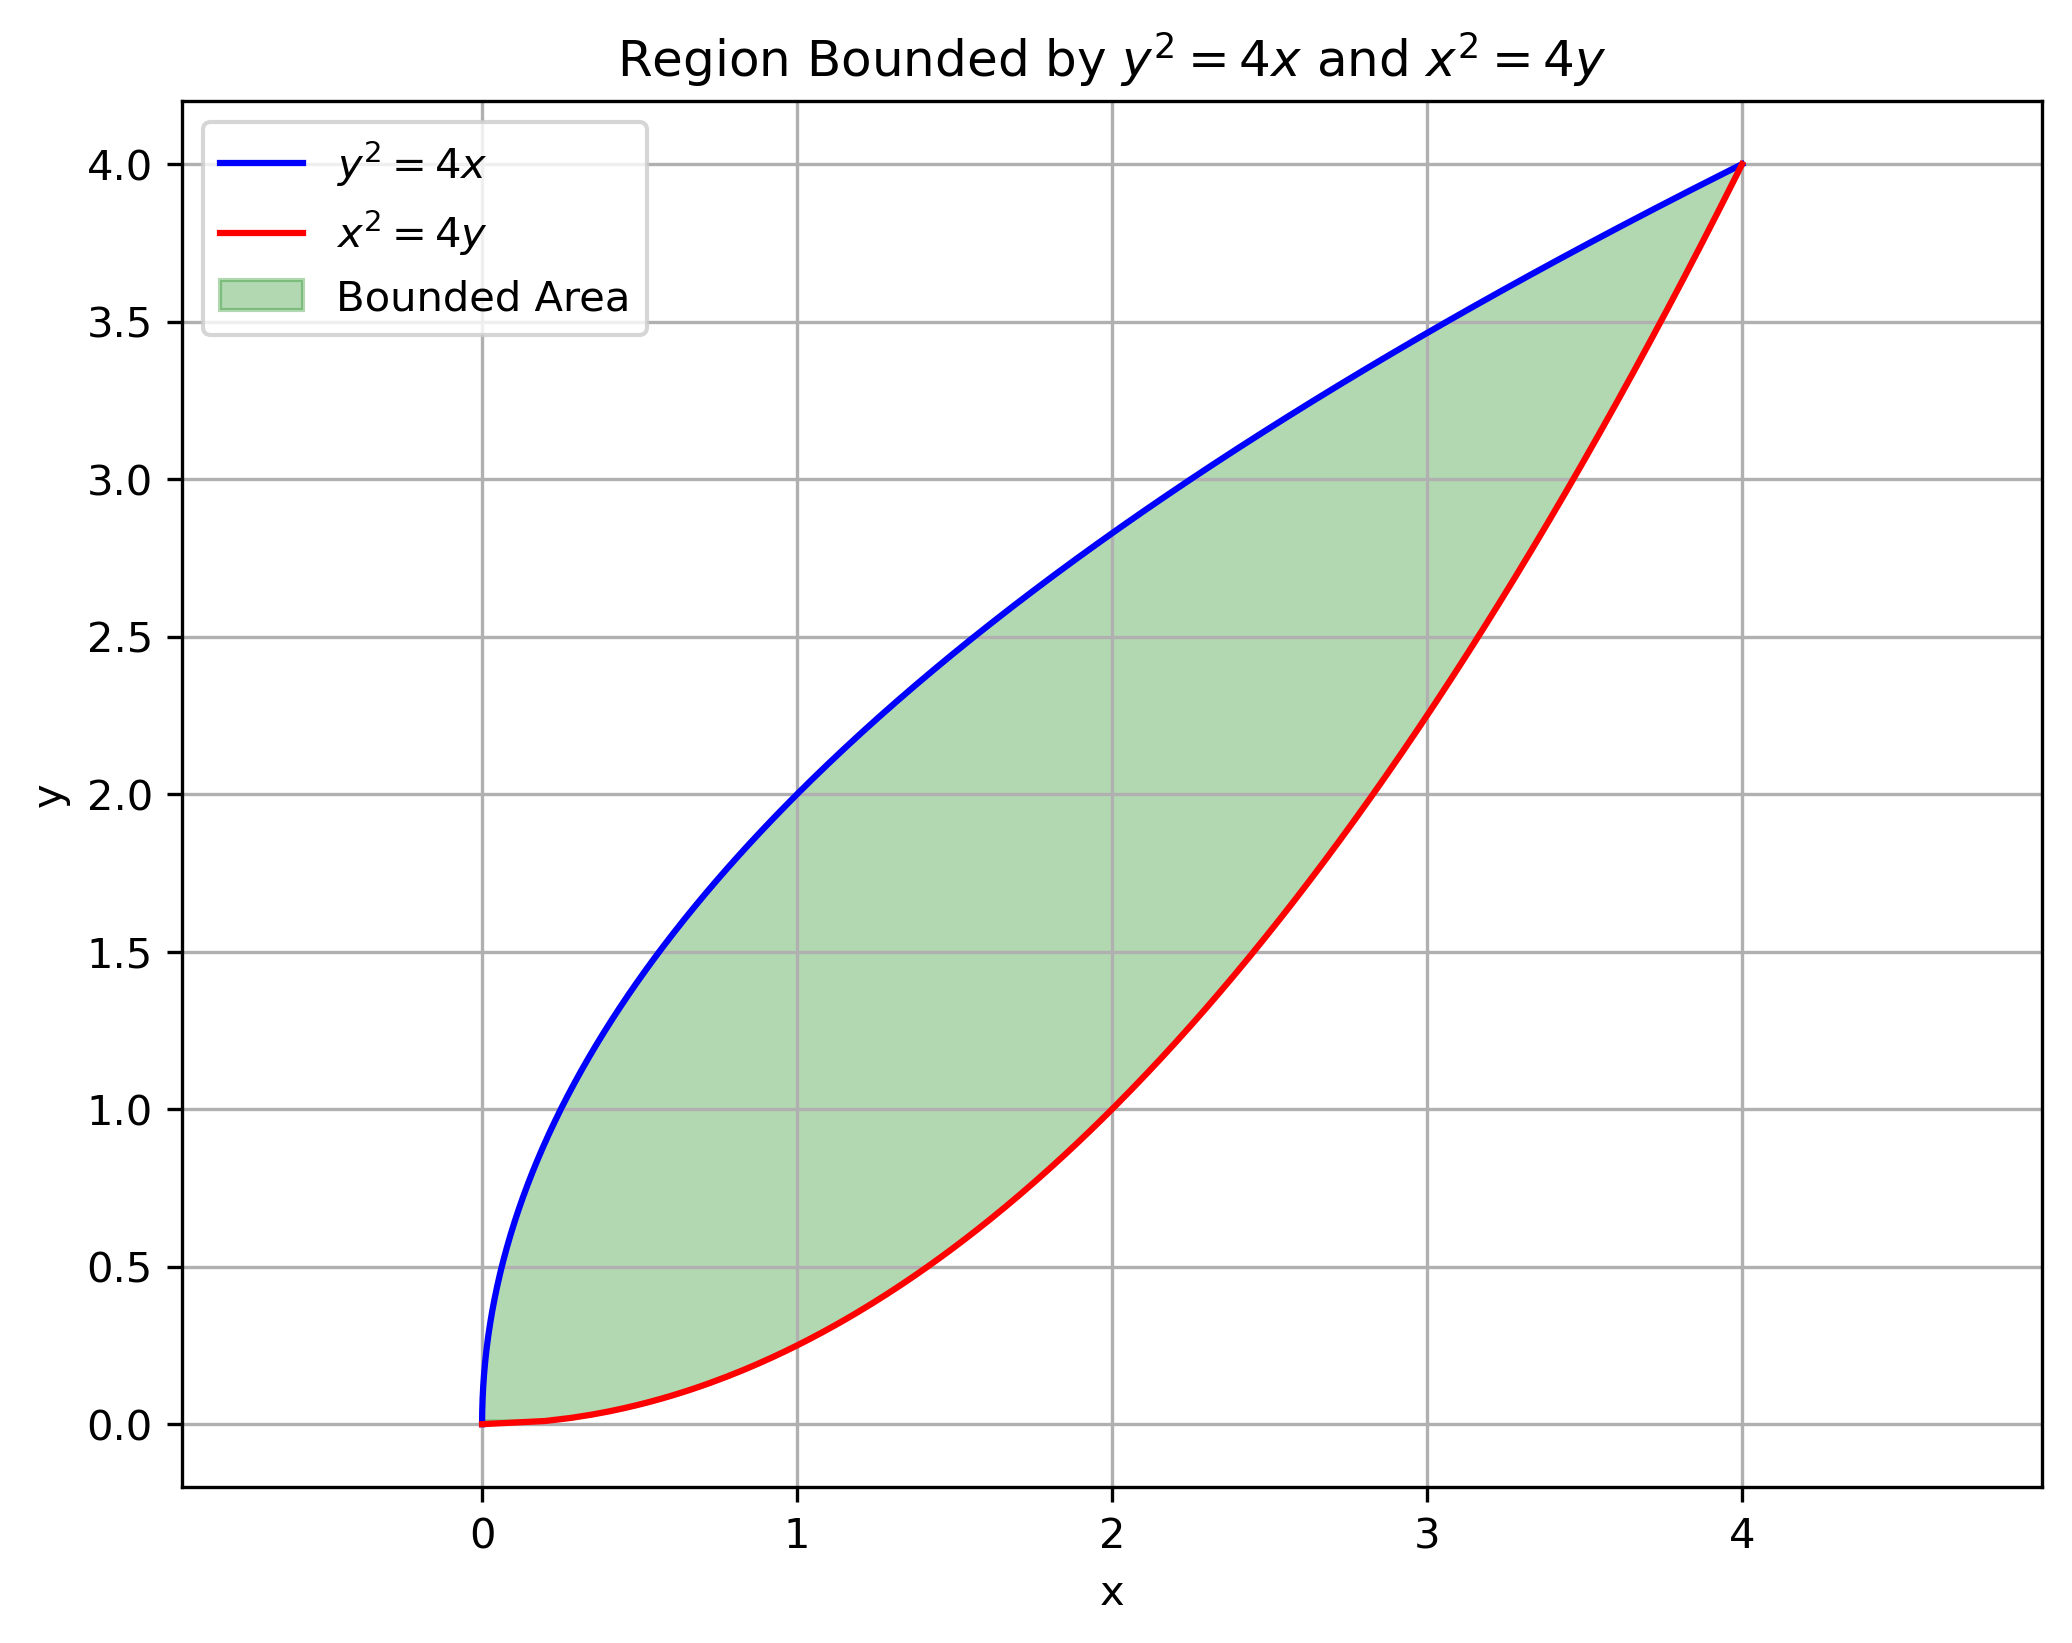
\includegraphics[width=0.7\linewidth]{figs/01.png}
    \caption{Area bounded}
    \label{fig:placeholder}
\end{figure}
\end{document}
